% This file is generated by the MATLAB m-file laprint.m. It can be included
% into LaTeX documents using the packages graphicx, color and psfrag.
% It is accompanied by a postscript file. A sample LaTeX file is:
%    \documentclass{article}\usepackage{graphicx,color,psfrag}
%    \begin{document}% This file is generated by the MATLAB m-file laprint.m. It can be included
% into LaTeX documents using the packages graphicx, color and psfrag.
% It is accompanied by a postscript file. A sample LaTeX file is:
%    \documentclass{article}\usepackage{graphicx,color,psfrag}
%    \begin{document}% This file is generated by the MATLAB m-file laprint.m. It can be included
% into LaTeX documents using the packages graphicx, color and psfrag.
% It is accompanied by a postscript file. A sample LaTeX file is:
%    \documentclass{article}\usepackage{graphicx,color,psfrag}
%    \begin{document}% This file is generated by the MATLAB m-file laprint.m. It can be included
% into LaTeX documents using the packages graphicx, color and psfrag.
% It is accompanied by a postscript file. A sample LaTeX file is:
%    \documentclass{article}\usepackage{graphicx,color,psfrag}
%    \begin{document}\input{ConHeli}\end{document}
% See http://www.mathworks.de/matlabcentral/fileexchange/loadFile.do?objectId=4638
% for recent versions of laprint.m.
%
% created by:           LaPrint version 3.15 (29.4.2004)
% created on:           21-Feb-2008 02:05:21
% eps bounding box:     15 cm x 11.25 cm
% comment:              
%
\begin{psfrags}%
\psfragscanon%
%
% text strings:
\psfrag{s03}[t][t]{\setlength{\tabcolsep}{0pt}\begin{tabular}{c}$x_1$\end{tabular}}%
\psfrag{s04}[b][b]{\setlength{\tabcolsep}{0pt}\begin{tabular}{c}$x_2$\end{tabular}}%
%
% xticklabels:
\psfrag{x01}[t][t]{-3}%
\psfrag{x02}[t][t]{-2}%
\psfrag{x03}[t][t]{-1}%
\psfrag{x04}[t][t]{0}%
\psfrag{x05}[t][t]{1}%
\psfrag{x06}[t][t]{2}%
\psfrag{x07}[t][t]{3}%
%
% yticklabels:
\psfrag{v01}[r][r]{-2}%
\psfrag{v02}[r][r]{-1.5}%
\psfrag{v03}[r][r]{-1}%
\psfrag{v04}[r][r]{-0.5}%
\psfrag{v05}[r][r]{0}%
\psfrag{v06}[r][r]{0.5}%
\psfrag{v07}[r][r]{1}%
\psfrag{v08}[r][r]{1.5}%
\psfrag{v09}[r][r]{2}%
%
% Figure:
\resizebox{12cm}{!}{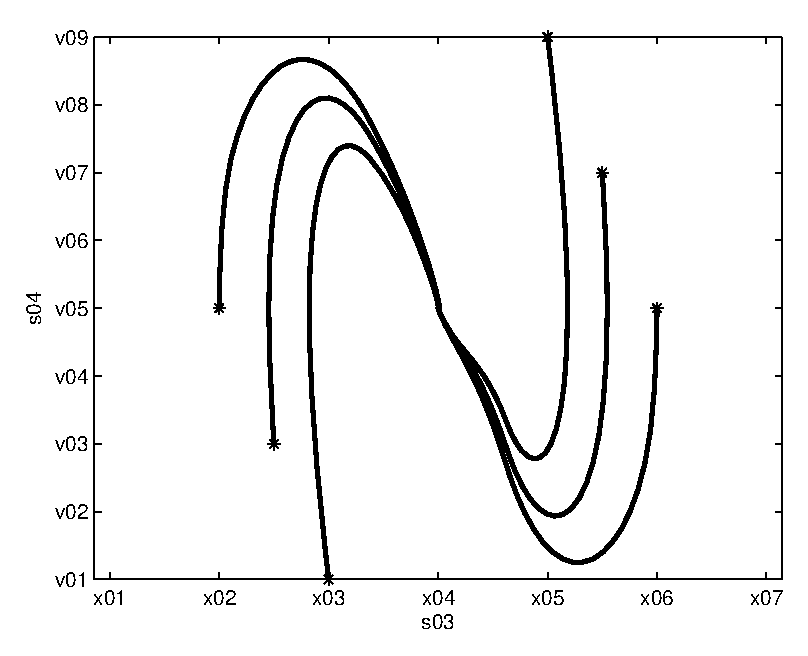
\includegraphics{images/ConHeli.eps}}%
\end{psfrags}%
%
% End ConHeli.tex
\end{document}
% See http://www.mathworks.de/matlabcentral/fileexchange/loadFile.do?objectId=4638
% for recent versions of laprint.m.
%
% created by:           LaPrint version 3.15 (29.4.2004)
% created on:           21-Feb-2008 02:05:21
% eps bounding box:     15 cm x 11.25 cm
% comment:              
%
\begin{psfrags}%
\psfragscanon%
%
% text strings:
\psfrag{s03}[t][t]{\setlength{\tabcolsep}{0pt}\begin{tabular}{c}$x_1$\end{tabular}}%
\psfrag{s04}[b][b]{\setlength{\tabcolsep}{0pt}\begin{tabular}{c}$x_2$\end{tabular}}%
%
% xticklabels:
\psfrag{x01}[t][t]{-3}%
\psfrag{x02}[t][t]{-2}%
\psfrag{x03}[t][t]{-1}%
\psfrag{x04}[t][t]{0}%
\psfrag{x05}[t][t]{1}%
\psfrag{x06}[t][t]{2}%
\psfrag{x07}[t][t]{3}%
%
% yticklabels:
\psfrag{v01}[r][r]{-2}%
\psfrag{v02}[r][r]{-1.5}%
\psfrag{v03}[r][r]{-1}%
\psfrag{v04}[r][r]{-0.5}%
\psfrag{v05}[r][r]{0}%
\psfrag{v06}[r][r]{0.5}%
\psfrag{v07}[r][r]{1}%
\psfrag{v08}[r][r]{1.5}%
\psfrag{v09}[r][r]{2}%
%
% Figure:
\resizebox{12cm}{!}{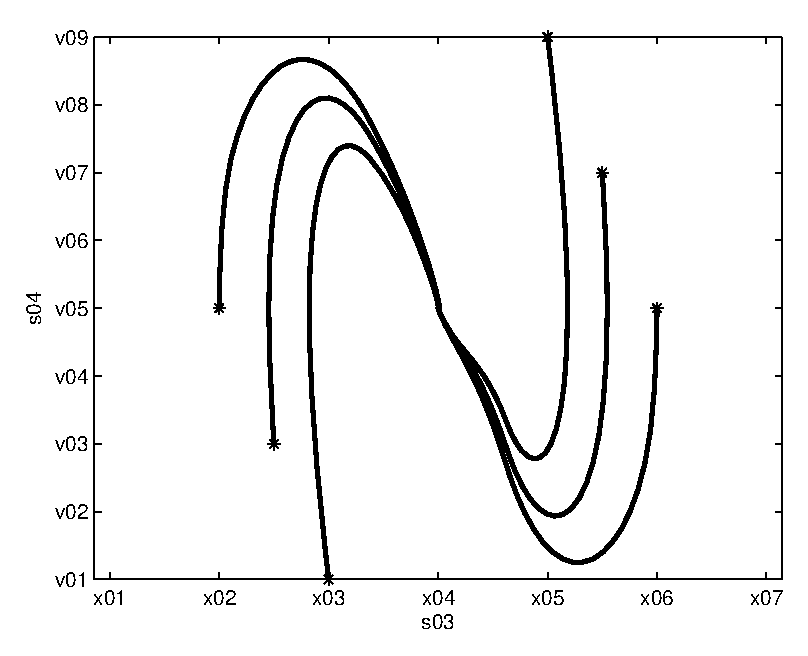
\includegraphics{images/ConHeli.eps}}%
\end{psfrags}%
%
% End ConHeli.tex
\end{document}
% See http://www.mathworks.de/matlabcentral/fileexchange/loadFile.do?objectId=4638
% for recent versions of laprint.m.
%
% created by:           LaPrint version 3.15 (29.4.2004)
% created on:           21-Feb-2008 02:05:21
% eps bounding box:     15 cm x 11.25 cm
% comment:              
%
\begin{psfrags}%
\psfragscanon%
%
% text strings:
\psfrag{s03}[t][t]{\setlength{\tabcolsep}{0pt}\begin{tabular}{c}$x_1$\end{tabular}}%
\psfrag{s04}[b][b]{\setlength{\tabcolsep}{0pt}\begin{tabular}{c}$x_2$\end{tabular}}%
%
% xticklabels:
\psfrag{x01}[t][t]{-3}%
\psfrag{x02}[t][t]{-2}%
\psfrag{x03}[t][t]{-1}%
\psfrag{x04}[t][t]{0}%
\psfrag{x05}[t][t]{1}%
\psfrag{x06}[t][t]{2}%
\psfrag{x07}[t][t]{3}%
%
% yticklabels:
\psfrag{v01}[r][r]{-2}%
\psfrag{v02}[r][r]{-1.5}%
\psfrag{v03}[r][r]{-1}%
\psfrag{v04}[r][r]{-0.5}%
\psfrag{v05}[r][r]{0}%
\psfrag{v06}[r][r]{0.5}%
\psfrag{v07}[r][r]{1}%
\psfrag{v08}[r][r]{1.5}%
\psfrag{v09}[r][r]{2}%
%
% Figure:
\resizebox{12cm}{!}{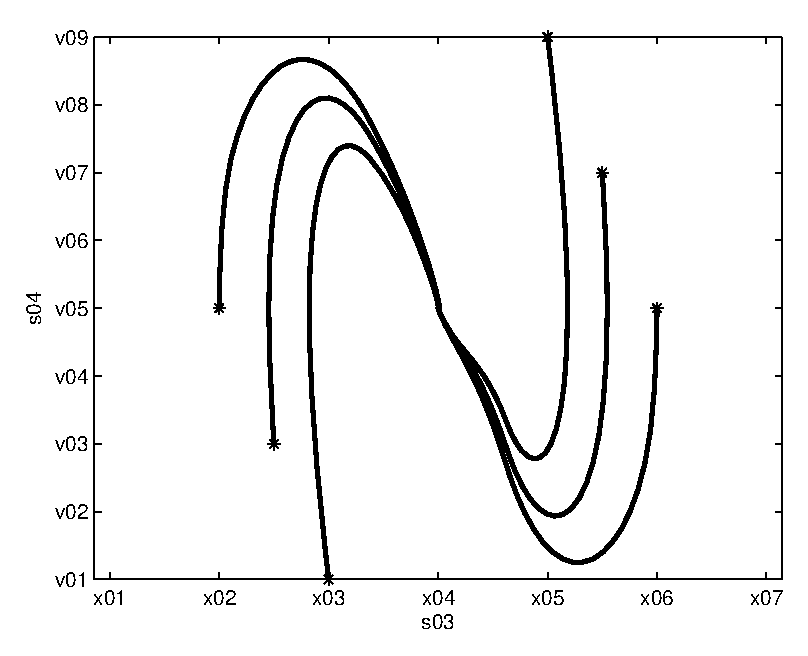
\includegraphics{images/ConHeli.eps}}%
\end{psfrags}%
%
% End ConHeli.tex
\end{document}
% See http://www.mathworks.de/matlabcentral/fileexchange/loadFile.do?objectId=4638
% for recent versions of laprint.m.
%
% created by:           LaPrint version 3.15 (29.4.2004)
% created on:           21-Feb-2008 02:05:21
% eps bounding box:     15 cm x 11.25 cm
% comment:              
%
\begin{psfrags}%
\psfragscanon%
%
% text strings:
\psfrag{s03}[t][t]{\setlength{\tabcolsep}{0pt}\begin{tabular}{c}$x_1$\end{tabular}}%
\psfrag{s04}[b][b]{\setlength{\tabcolsep}{0pt}\begin{tabular}{c}$x_2$\end{tabular}}%
%
% xticklabels:
\psfrag{x01}[t][t]{-3}%
\psfrag{x02}[t][t]{-2}%
\psfrag{x03}[t][t]{-1}%
\psfrag{x04}[t][t]{0}%
\psfrag{x05}[t][t]{1}%
\psfrag{x06}[t][t]{2}%
\psfrag{x07}[t][t]{3}%
%
% yticklabels:
\psfrag{v01}[r][r]{-2}%
\psfrag{v02}[r][r]{-1.5}%
\psfrag{v03}[r][r]{-1}%
\psfrag{v04}[r][r]{-0.5}%
\psfrag{v05}[r][r]{0}%
\psfrag{v06}[r][r]{0.5}%
\psfrag{v07}[r][r]{1}%
\psfrag{v08}[r][r]{1.5}%
\psfrag{v09}[r][r]{2}%
%
% Figure:
\resizebox{12cm}{!}{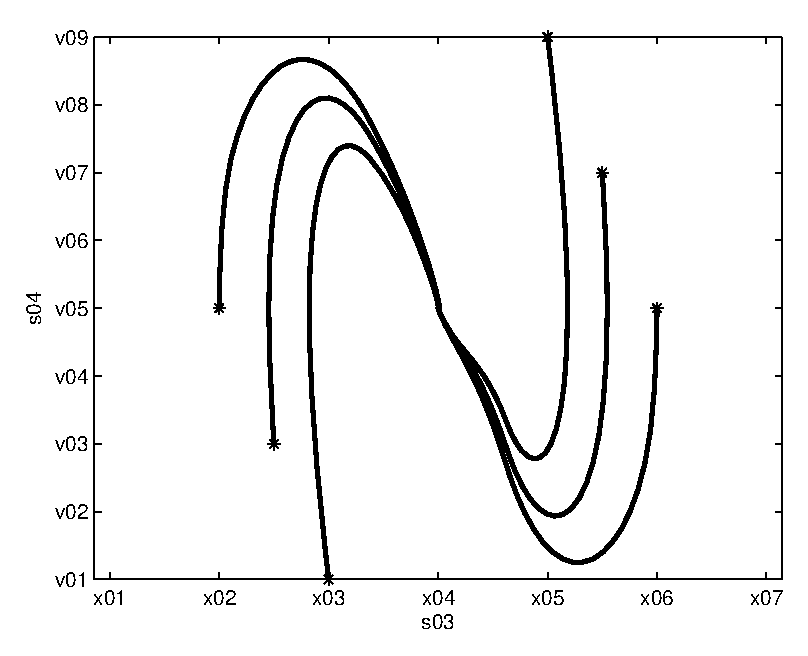
\includegraphics{images/ConHeli.eps}}%
\end{psfrags}%
%
% End ConHeli.tex
